\documentclass[11pt]{article}
 
\usepackage[margin=1in]{geometry} 
\usepackage{amsmath,amsthm,amssymb}
\usepackage{graphicx} 
\usepackage{blkarray}
\usepackage{amsmath}




\newcommand{\N}{\mathbb{N}}
\newcommand{\Z}{\mathbb{Z}}
 
\newenvironment{problem}[2][Problem]{\begin{trivlist}
\item[\hskip \labelsep {\bfseries #1}\hskip \labelsep {\bfseries #2.}]}{\end{trivlist}}
\newenvironment{lemma}[2][Lemma]{\begin{trivlist}
\item[\hskip \labelsep {\bfseries #1}\hskip \labelsep {\bfseries #2.}]}{\end{trivlist}}
\newenvironment{exercise}[2][Exercise]{\begin{trivlist}
\item[\hskip \labelsep {\bfseries #1}\hskip \labelsep {\bfseries #2.}]}{\end{trivlist}}

\newenvironment{question}[2][Question]{\begin{trivlist}
\item[\hskip \labelsep {\bfseries #1}\hskip \labelsep {\bfseries #2.}]}{\end{trivlist}}
\newenvironment{corollary}[2][Corollary]{\begin{trivlist}
\item[\hskip \labelsep {\bfseries #1}\hskip \labelsep {\bfseries #2.}]}{\end{trivlist}}

\usepackage{indentfirst}
\linespread{1.2}     % 调整间距
\setlength{\parindent}{0pt}

\begin{document}

 
% --------------------------------------------------------------
%                         Start here
% --------------------------------------------------------------
 
\title{Homework 5 DS-GA 1002 }%replace X with the appropriate number
\author{Yuhao Zhao\\ %replace with your name
N17578783} %if necessary, replace with your course title
 
\maketitle
\begin{problem}{1}
\end{problem}
(a) Assuming that each bet is independent of others, Let $X_i$ be the Bernoulli distribution with $X_i = 1$ if getting the right number. Then $X(x) = \sum_{i  =1}^{100} X_i \sim Binomial(100,x) $ with $p = \frac{1}{38}$\\
By CLT, $X \to^d N(\frac{100}{38}, 100\frac{37}{38^2})\approx N(2.632,2.562)$\\
If Bob is making money, let the number of wining be $x, x$ must satisfy $36x-100>0,x> \frac{100}{36} $\\
$P(X\geq\frac{100}{36}) = 1- P(X\leq\frac{100}{36}) = 1- P(\frac{X - \frac{100}{38}}{\sqrt{ 100\frac{37}{38^2}}} \leq \frac{\frac{100}{36} - \frac{100}{38}}{\sqrt{ 100\frac{37}{38^2}}}) = 1 - P(Z< 0.2302) \approx  0.4636$\\

(b) Let $Y_i$ be the Bernoulli distribution with $Y_i = 1$ if getting the right color. Then $Y(y) = \sum_{i  =1}^{100} Y_i \sim Binomial(100,y) $ with $p = \frac{18}{38}$\\
 By CLT, $Y \to^d N(\frac{100\times 18}{38}, 100\frac{18\times 20}{38^2}) \approx N(47.368, 24.931)$\\
 If Bob is making money, let the number of wining be $y, y$ must satisfy $2y-100>0,y> 50 $\\
$P(Y>50) = 1- P(Y > 50) = 1- P(\frac{Y -\frac{100\times 18}{38} }{\sqrt{ 100\frac{18\times 20}{38^2}}} \leq \frac{50 -\frac{100\times 18}{38}}{\sqrt{ 100\frac{18\times 20}{38^2}}}) = 1 - P(Z< 0.7273) \approx 0.2991$\\

(c) By CLT, for n goes to infinity, for betting on numbers, the expectation  is  $\frac{100}{38} \times 36 - 100 = - \frac{100}{19}$\\
 for betting on color, the expectation  is  $\frac{100*18}{38} \times 2 - 100 = - \frac{100}{19}$\\
 Therefore, he is expected to lose money finally.\\
 However, $sd(36X) \approx 78$ $>sd(2Y)  \approx 78 \approx  9$ \\
betting on colors is asymptotically better\\


(d)$P(X=x|x \geq \frac{100}{36}) = \frac{P(X= x)}{0.4636}, E(X|x \geq \frac{100}{36}) = \int_{\frac{100}{36}}^{\infty} \frac{xf(x)}{0.4636}dx \\= \int_{\frac{100}{36}}^{\infty} \frac{xe^{-\frac{(x - 2.632)^2}{2\times2.562}}}{\sqrt{2\times 2.562 \times \pi}} \times \frac{1}{0.4636}dx \approx  4.0043  $\\
The expected gain is $4.0043\times 36 -100 \approx 44.1548$\\
$P(Y=y|y \geq 50) = \frac{P(Y= y)}{0.2991}, E(Y|y \geq 50) = \int_{50}^{\infty} \frac{xf(x)}{0.2991}dx = \int_{50}^{\infty} \frac{xe^{-\frac{(x - 47.368)^2}{2\times24.931}}}{\sqrt{2\times 24.931 \times \pi}} \times \frac{1}{0.2991}dx \approx  53.156  $\\
The expected gain is $ 53.156\times 2 -100 \approx 6.312$\\
Therefore, he will choose betting on the numbers. The expected gain is 44.1548\\

\pagebreak

\begin{problem}{2}
\end{problem}
(a) Since we know that the maximum of weight is 1400lbs. the max sd is 1400.\\
By the confidence interval for variables with bounded variance, we know that:\\ $P(\mu \in [\bar{X_n} - \frac{b}{\sqrt{\alpha n}},\bar{X_n} + \frac{b}{\sqrt{\alpha n}}])\geq 1- \alpha$, $\sigma x_i \leq b$\\
we set b = 1400, and $\alpha  = 0.05$\\
$\frac{1400}{\sqrt{0.05\times n}} \leq 2.5, n\geq 6272000$\\
So we need to sample 1568000 individuals.\\

(b) Assuming n =1000 is enough for the sample variance to be closed to the true variance ,from the asymptotic confidence interval fro the sample mean:\\
$P(\mu \in [\bar{X_n} - \frac{\hat{\sigma}}{\sqrt{n}}Q^{-1}(\frac{\alpha}{2}),\bar{X_n} + \frac{\hat{\sigma}}{\sqrt{n}}Q^{-1}(\frac{\alpha}{2})] \approx 1- \alpha$\\
$\frac{\sqrt{144}}{\sqrt{n}} \times 1.96 \leq 2.5, n\geq 88$\\\
So we need at least 88 individuals.\\

(c) For n = 20, 0 intervals out of 10000 don't contain the true mean. For n = 1000,0 intervals out of 10000 don't contain the true mean. This means the confidence interval is precise for both n = 20 and n = 1000\\
The true variance of the weights are 135.97. For n =20, the distribution of sample variance is biased and heavy tailed. This means that the variance calculated from 20 sample is not enough to estimate the true sample variance. For n = 1000, the distribution of variance is unbiased and light tailed. Therefore using sample variance of 1000 data is a close to the true variance.  \\

\begin{question}{3}
\end{question}
(a)We want to show: $P(A\leq a- \epsilon) - P(|A_n - A |> \epsilon) \leq P(A_n \leq a ) \leq P(A\leq a+ \epsilon) + P(|A_n - A| > \epsilon)$\\
On the one hand, $P(A_n \leq a) = P(A_n \leq a,A\leq a+\epsilon)+P(A_n \leq a, A \geq a+\epsilon)$\\
$\leq P(A \leq a+ \epsilon) + P(A_n - A \leq a- A, a -A \leq -\epsilon) \leq P(A \leq a+ \epsilon)  + P(A_n -A \leq -\epsilon)\\ \leq P(A \leq a+ \epsilon) + P(A_n -A \leq -\epsilon)  + P(A_n -A \geq \epsilon) = P(A\leq a+ \epsilon) + P(|A_n - A| > \epsilon)$\\
On the other hand, $P(A\leq a - \epsilon) = P(A\leq a - \epsilon ,A_n \leq \epsilon +A )+ P(A\leq a - \epsilon ,A_n \geq \epsilon +A ) \\
= P(A_n\leq \epsilon+A, A+\epsilon \leq a) +   P(A\leq a - \epsilon ,A_n \geq \epsilon +A ) \leq P(A_n \leq a)+ P(An_a \leq \epsilon)$\\
$\leq  P(A_n \leq a)+ P(A_n-A \geq \epsilon) + P(A_n -A\leq -\epsilon) = P(A_n \leq a )+ P(|A_n -A |\geq \epsilon)$\\
Therefore, $P(A_n \leq a) \geq P(A\leq a - \epsilon) - P(|A_n -A |\geq \epsilon) $\\
These two inequalities shows $P(A\leq a- \epsilon) - P(|A_n - A |> \epsilon) \leq P(A_n \leq a ) \leq P(A\leq a+ \epsilon) + P(|A_n - A| > \epsilon)$\\

(b) Since $A_n \to A$ in probability, $\forall \epsilon > 0, \lim\limits_{n \to \infty } P(|A_n-A| >\epsilon ) = 0$\\
From (a), $P(A\leq a- \epsilon) - P(|A_n - A |> \epsilon)\leq P(A_n \leq a)  \leq P(A\leq a+ \epsilon) + P(|A_n - A| > \epsilon)$\\
This yields, $P(A\leq a- \epsilon) \leq P(A_n \leq a)  \leq P(A\leq a+\epsilon) \Longleftrightarrow F_A(a- \epsilon) \leq P(A_n \leq a) \leq F_A(a+\epsilon) $  \\
Since $\epsilon$ is an arbitrary number, this means $F_A(a) = F_{A_n}(a), \lim\limits_{n \to \infty} P(A_n\leq a) = P(A \leq a)$\\
By definition $A_n$ converge to A in distribution.\\

(c) Converge in distribution does not imply converge in probability. A counterexample is $X ~ N(0,1), X_n = -X$, $X_n $ and $X$ has the same cdf but they don't converge in probability.    


\begin{problem}{4}
\end{problem}
(a)

\begin{centering}
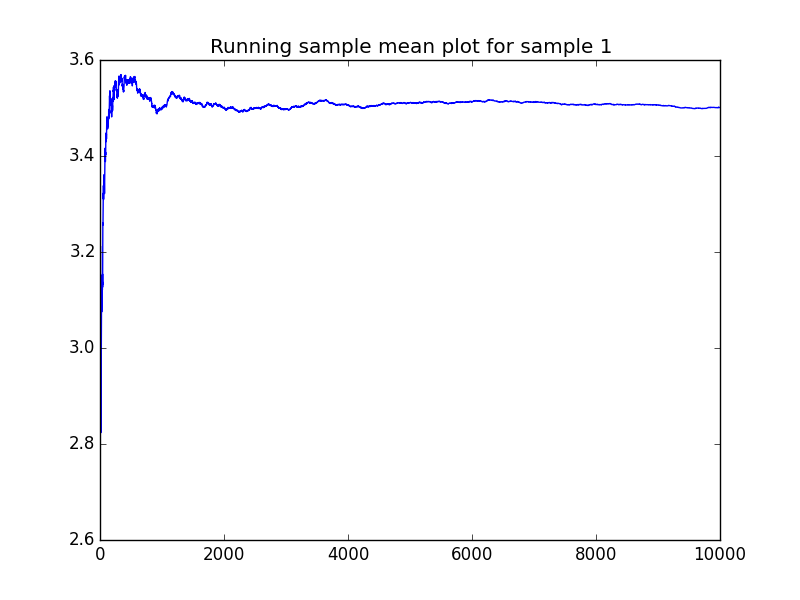
\includegraphics[height = 3.3in]{Q4_a} 

\end{centering}

A reasonable estimator for c can be 3.5. This method will work only if the mean and variance of the sample is well defined and finite.\\
(b)

\begin{centering}
	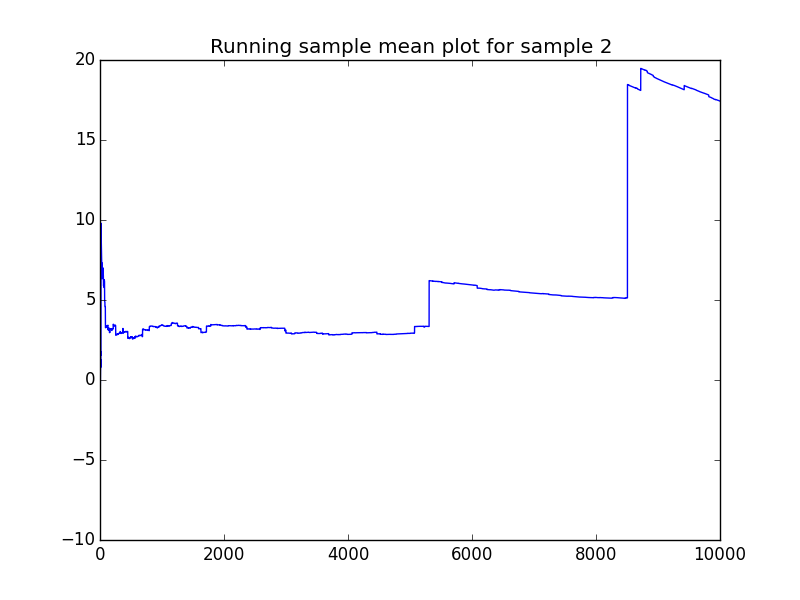
\includegraphics[height = 3.3in]{Q4_b} 
	
\end{centering}
The method does't work. There are extremely large data point such that the running mean does not seems to converge.\\



(c) $\alpha$ is uniformly distributed from [$-\pi/2, \pi/2$], $P(X \in [0,x]) = \int_{0}^{\arctan(x)} \frac{1}{\pi} d\alpha = \frac{\arctan(x)}{\pi}$\\
$f(x) = d \frac{\arctan(x)}{\pi}/dx = \frac{1}{\pi(1+x^2)}$\\
$E(x) = \int_{-\infty}^{\infty}\frac{x}{\pi(1+x^2) }dx = \int_{-\infty}^{\infty}\frac{1}{2\pi(1+x^2) }dx^2  = \int_{0}^{\infty}\frac{1}{2\pi(1+t) }dt = \frac{log(t+1)}{2\pi} |_{0}^{\infty} = \infty$\\
Therefore the mean of X is not defined.Therefore, for this random variable, Law of large number doesn't work.This model can explain our observation.\\

(d)We can sample points from $\alpha \sim unif[-\pi/2, \pi/2]$, and transform to x by $x = tan(\alpha)$

\begin{centering}
	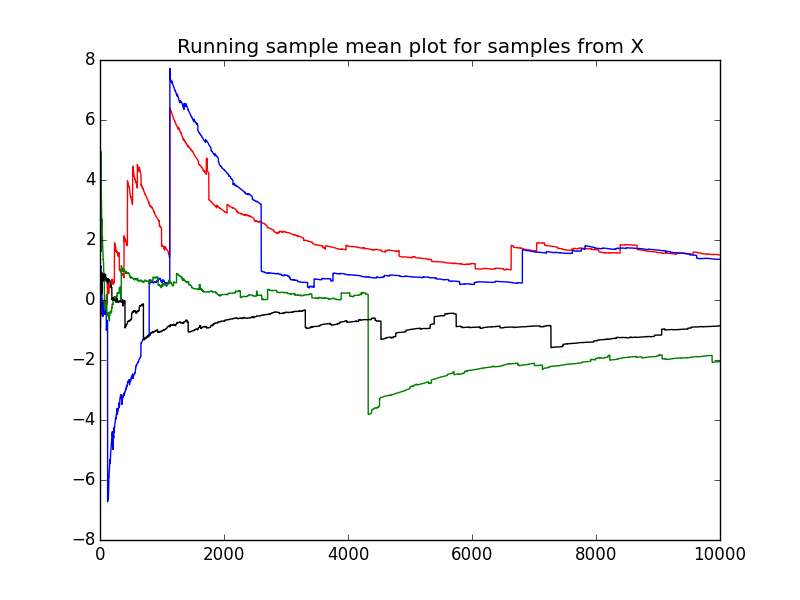
\includegraphics[height = 3.3in]{Q4_c} 
	
\end{centering}
From the plots, it's clear that the sample means do not converge to the same value. LLN fails.\\

\begin{problem}{5}
\end{problem}
(a) If the sample mean is greater than 0.5 then the Republican is more likely to win the election. Otherwise, the Democrat is more likely to win. This will work when the sample is randomly selected and are iid, and the number of sample is sufficiently large.\\

(b)% Since $P(\mu \in [\bar{R_n} - \frac{b}{\sqrt{\alpha n}},\bar{R_n} + \frac{b}{\sqrt{\alpha n}}])\geq 1- \alpha$, $\sigma R_i \leq b$, in this case R is a Bernoulli, b = 1.\\
Since $R_i$ is Bernoulli distribution, $Var(R_i)  = p(1 - p) \leq \frac{1}{4}$\\
From the sample , $\bar{R}_n = 45/94 < \frac{1}{2}$,the Democrat will win the election.\\
By Chebyshev's inequality: $P(|\bar{R}_n - p| \geq \alpha) \leq \frac{Var(\bar{R}_n)}{\alpha^2} = \frac{1}{4n} \frac{1}{\alpha^2}$\\
$P(|\bar{R}_n - p| \geq \alpha) \geq P(p \geq \bar{R}_n+ \alpha ) = P(p \geq \frac{45}{94} + \alpha)$\\
Let $\alpha = \frac{1}{2} - \frac{45}{94}$, we have $P(p>\frac{1}{2}) \leq \frac{1}{4\times 94000 \times(\frac{1}{2} - \frac{45}{94})^2 } \approx 0.005875$

It does not mean that it's an upper bound of the probability that the prediction is right. \\

(c) Let $n_{Y,R}$ be the number of young people vote for Republican, $n_{Y,D}$ the number of young people vote for Democrat, $n_{O,R}$ be the number of old people vote for Republican, $n_{O,D}$ the number of young people vote for Democrat.\\
$E(X_{n_1,n_2}) = a E(\sum_{n_1} Y_i) + bE(\sum_{n_2} O_i) = \frac{n_{Y,R}+ n_{Y,D} }{n_{Y,R}+n_{Y,D}+n_{O,R}+n_{O,D}}\times \mu_Y + \frac{n_{O,R}+ n_{O,D}}{n_{Y,R}+n_{Y,D}+n_{O,R}+n_{O,D}}\times \mu_O$\\
$E(\sum_{n_1} Y_i) = n_1 \mu_Y, E(\sum_{n_2} O_i) = n_2\mu_O$\\
Therefore, $a =  \frac{n_{Y,R} + n_{Y,D}}{n_{Y,R}+n_{Y,D}+n_{O,R}+n_{O,D}} \times \frac{1}{n_1}, b = \frac{n_{O,R}+ n_{O,D}}{n_{Y,R}+n_{Y,D}+n_{O,R}+n_{O,D}}\times \frac{1}{n_2} $\\

(d) From (c) $X_{59000,35000} = \frac{0.2}{0.2+0.55} \times \frac{24000}{59000} + \frac{0.55}{0.2+0.55} \times \frac{21000}{35000} =\frac{809}{1475} \approx 0.5799031 > 0.5$\\
We predict that Republican will win the election\\
We assume that  the sample for both groups are selected randomly. Within each group the data are i.i.d\\%$Sd(X_{n_1,n_2}) \leq 1$, the 95\% confidence interval is :\\ $[0.5799031-\frac{1}{\sqrt{0.05 \times (35000+59000)}} ,0.5799031+\frac{1}{\sqrt{0.05 \times (35000+59000)}}] = [0.5653135, 0.5944865]$\\
$Var(X_{n_1,n_2})  \leq a^2\times n_1\times \frac{1}{4} + b^2 \times n_2 \times \frac{1}{4} = \frac{1}{4}(\frac{4}{15}^2 \frac{1}{59000} + \frac{11}{15}^2 \frac{1}{35000})$\\
By Chebyshev's inequality: $P(|\bar{X}_{n_1,n_2}- p| \geq \alpha) \leq \frac{Var(\bar{X}_{n_1,n_2})}{\alpha^2} $\\
$P(|\bar{X}_{n_1,n_2}- p| \geq \alpha) \geq P(p \leq \bar{X}_{n_1,n_2} - \alpha  )$, let $\alpha = \frac{809}{1475} - \frac{1}{2} $\\
$P(p \leq \frac{1}{2}  ) \leq \frac{1}{\alpha^2} \times \frac{1}{4}(\frac{4}{15}^2 \frac{1}{59000} + \frac{11}{15}^2 \frac{1}{35000}) \approx 0.001763$

%Since the interval doesn't cover 0.5, we predict that Republican will win the election.\\
%The assumption is that the sample for both groups are selected randomly. 
 


 







\end{document}